% ============================================================
%  RAPPORT DE STAGE S8 — Adrien Collignon
%  ACDC Research Group, UNSW Sydney, mars–août 2025
%  Compiler : pdfLaTeX + biber  (Overleaf : pdfLaTeX recommandé)
% ============================================================
\documentclass[12pt,a4paper]{report}

% ── Encodage & langue ──────────────────────────────────────
\usepackage[utf8]{inputenc}
\usepackage[T1]{fontenc}
\usepackage[french]{babel}
\usepackage{csquotes}

% ── Mise en page ───────────────────────────────────────────
\usepackage[top=2.5cm,bottom=2.5cm,left=2.8cm,right=2.8cm,headheight=15pt]{geometry}
\usepackage{fancyhdr}
\usepackage{emptypage}
\usepackage{setspace}
\onehalfspacing

% ── Police : EB Garamond (disponible sur Overleaf) ─────────
\usepackage{ebgaramond}
\usepackage[scaled=0.85]{beramono}

% ── Couleurs ───────────────────────────────────────────────
\usepackage{xcolor}
\definecolor{orange}{HTML}{C55A11}
\definecolor{warmwhite}{HTML}{FFF8F0}
\definecolor{lightblue}{HTML}{EBF4FA}

% ── Titres ─────────────────────────────────────────────────
\usepackage{titlesec}
\titleformat{\chapter}[display]
  {\normalfont\huge\bfseries\color{orange}}
  {\chaptertitlename\ \thechapter}{10pt}{\Huge}
\titleformat{\section}
  {\normalfont\Large\bfseries}{\thesection}{1em}{}
\titleformat{\subsection}
  {\normalfont\large\bfseries\color{orange}}{\thesubsection}{1em}{}
\titleformat{\subsubsection}
  {\normalfont\normalsize\bfseries}{\thesubsubsection}{1em}{}
\titlespacing*{\chapter}{0pt}{-10pt}{20pt}

% ── TDM ────────────────────────────────────────────────────
\usepackage[titles]{tocloft}
\setlength{\cftbeforechapskip}{4pt}

% ── Maths ──────────────────────────────────────────────────
\usepackage{amsmath,amssymb}
\usepackage{siunitx}
\sisetup{locale=FR,per-mode=symbol}

% ── Figures & tableaux ─────────────────────────────────────
\usepackage{graphicx}
\usepackage{float}
\usepackage{caption}
\usepackage{subcaption}
\usepackage{booktabs}
\usepackage{tabularx}
\usepackage{array}
\usepackage{longtable}
\captionsetup{font=small,labelfont=bf}
\graphicspath{{figures/}}

% ── Encadrés ───────────────────────────────────────────────
\usepackage{tcolorbox}
\tcbuselibrary{breakable,skins}
\newtcolorbox{encadre}[1][]{
  colback=warmwhite,colframe=orange,arc=3pt,
  leftrule=3pt,rightrule=0.5pt,toprule=0.5pt,bottomrule=0.5pt,
  fonttitle=\bfseries\color{orange},#1}
\newtcolorbox{infobox}[1][]{
  colback=lightblue,colframe=blue!40!black,arc=3pt,
  leftrule=3pt,fonttitle=\bfseries,#1}

% ── Listes ─────────────────────────────────────────────────
\usepackage{enumitem}
\setlist[itemize]{itemsep=2pt,topsep=4pt}

% ── Liens ──────────────────────────────────────────────────
\usepackage[colorlinks,linkcolor=orange,citecolor=orange,urlcolor=orange,
  pdftitle={Rapport de stage S8 — Adrien Collignon},
  pdfauthor={Adrien Collignon}]{hyperref}

% ── Biblio ─────────────────────────────────────────────────
\usepackage[backend=biber,style=numeric,sorting=none]{biblatex}
\addbibresource{references.bib}

% ── Divers ─────────────────────────────────────────────────
\usepackage{microtype}
\usepackage{multicol}

% ── En-têtes ───────────────────────────────────────────────
\pagestyle{fancy}\fancyhf{}
\fancyhead[L]{\small\textit{Rapport de stage S8 — Adrien Collignon}}
\fancyhead[R]{\small\textit{\leftmark}}
\fancyfoot[C]{\thepage}
\renewcommand{\headrulewidth}{0.4pt}

% ── Macros pratiques ───────────────────────────────────────
\newcommand{\ivoc}{$i$Voc}
\newcommand{\qfls}{QFLS}
\newcommand{\kTq}{\ensuremath{k_BT/q}}

% ============================================================
\begin{document}
% ============================================================

% ── PAGE DE GARDE ──────────────────────────────────────────
\begin{titlepage}
\thispagestyle{empty}
\begin{center}

\begin{minipage}{0.45\textwidth}
  
\includegraphics[height=2cm]{logo_centrale}
\end{minipage}\hfill
\begin{minipage}{0.45\textwidth}
  \raggedleft
\includegraphics[height=2cm]{logo_acdc}
\end{minipage}

\vspace{1cm}
{\large Rapport de stage S8 en semestre à Sydney, Australie}\\
{\large (de mars à août 2025)}

\vspace{1.2cm}
\rule{\linewidth}{1.5pt}\\[0.4cm]
{\Huge\bfseries\color{orange}
  Extraction de l'$i$Voc en conditions\\[0.2cm]
  outdoor pour des échantillons III-V
}\\[0.3cm]
\rule{\linewidth}{1.5pt}

\vspace{1.2cm}
{\Large Adrien \textsc{Collignon}}\\[0.2cm]
{\large Élève ingénieur (2\textsuperscript{ème} année)}\\
{\large École Centrale Méditerranée — Promo entrante 2023}

\vspace{1.5cm}
\begin{minipage}{0.48\textwidth}
  \raggedright
  \textbf{Maître de stage :}\\
  M.\ Ziv \textsc{Hameiri}\\
  ACDC Research Group, UNSW Sydney
\end{minipage}\hfill
\begin{minipage}{0.48\textwidth}
  \raggedleft
  \textbf{Tuteur académique :}\\
  M.\ \textsc{Bourennane}\\
  École Centrale Méditerranée
\end{minipage}

\vfill
{\large ACDC Research Group\\
School of Photovoltaic \& Renewable Energy Engineering\\
UNSW Sydney, Kensington NSW 2052, Australie\\[0.3cm]
2025}
\end{center}
\end{titlepage}

% ── REMERCIEMENTS ──────────────────────────────────────────
\chapter*{Remerciements}
\addcontentsline{toc}{chapter}{Remerciements}

Je souhaite tout d'abord remercier chaleureusement le Professeur Ziv Hameiri, mon tuteur de stage au sein de l'Université de Nouvelle-Galles du Sud (UNSW), pour son accueil attentif, son accompagnement tout au long du stage et sa confiance dans la conduite autonome de mon projet. Sa rigueur scientifique, sa bienveillance et son implication dans la vie du groupe ont grandement contribué à la qualité de mon expérience.

Je tiens également à exprimer ma profonde gratitude à l'ensemble des membres de l'ACDC Research Group, pour leur accueil chaleureux, leur bonne humeur constante et leur grande disponibilité. Grâce à eux, j'ai découvert un environnement de travail international, dynamique et stimulant, où la convivialité va de pair avec l'exigence scientifique.

Je remercie aussi les autres étudiants et stagiaires présents au laboratoire, pour la qualité de nos échanges, l'entraide spontanée et le partage d'idées tout au long du stage.

Un mot de remerciement également à Monsieur Bourennane, tuteur académique à l'École Centrale Méditerranée, pour avoir accepté d'encadrer administrativement ce stage à distance, et pour sa réactivité lors de nos échanges.

Enfin, je remercie ma famille et mes proches pour leur soutien indéfectible dans cette expérience à l'étranger, et leur présence, même à distance, dans les moments de doute comme dans les réussites.

% ── RÉSUMÉ ─────────────────────────────────────────────────
\chapter*{Résumé -- Abstract}
\addcontentsline{toc}{chapter}{Résumé -- Abstract}

\section*{Résumé}
Ce rapport présente les travaux réalisés dans le cadre d'un stage de recherche de cinq mois au sein de l'ACDC Research Group, un laboratoire spécialisé dans les technologies photovoltaïques rattaché à l'Université de Nouvelle-Galles du Sud (UNSW), à Sydney (Australie).

Le projet porte sur l'extraction de la tension en circuit ouvert implied ($i$Voc) en conditions outdoor pour des échantillons de semi-conducteurs III-V. En autonomie, j'ai développé une méthodologie de mesure et d'analyse permettant de caractériser les propriétés de recombinaison de ces matériaux à hautes performances sous illumination solaire réelle.

\bigskip
\begin{otherlanguage}{english}
\section*{Abstract}
This report outlines the work carried out during a five-month research internship within the ACDC Research Group, a photovoltaics-focused laboratory based at the University of New South Wales (UNSW) in Sydney, Australia.

The project focused on the extraction of the implied open-circuit voltage ($i$Voc) under outdoor conditions for III-V semiconductor samples. Working independently, I developed a measurement and analysis methodology to characterise the recombination properties of these high-performance materials under real solar illumination.
\end{otherlanguage}

% ── GLOSSAIRE ──────────────────────────────────────────────
\chapter*{Glossaire}
\addcontentsline{toc}{chapter}{Glossaire}

\begin{tabularx}{\textwidth}{lX}
\toprule
\textbf{Terme} & \textbf{Définition} \\
\midrule
$i$Voc & Tension en circuit ouvert implicite, extraite à partir de mesures de photoluminescence sans contact électrique. \\[4pt]
III-V & Semi-conducteurs composés d'éléments des groupes III et V de la classification périodique (ex.\ GaAs, InP, GaInP). \\[4pt]
Photoluminescence (PL) & Émission de lumière par un matériau suite à une excitation optique. \\[4pt]
QFLS & Séparation des niveaux de quasi-Fermi (\textit{Quasi-Fermi Level Splitting}), directement liée à l'$i$Voc. \\[4pt]
Irradiance & Puissance solaire reçue par unité de surface, exprimée en \si{W/m^2}. \\[4pt]
\textit{Outdoor measurement} & Mesure réalisée sous illumination solaire naturelle, par opposition aux mesures indoor. \\[4pt]
Calibration & Procédure d'étalonnage des instruments de mesure pour garantir la fiabilité des résultats. \\[4pt]
Défaut cristallin & Imperfection dans la structure cristalline d'un semi-conducteur, source de recombinaison non radiative. \\[4pt]
Recombinaison non radiative & Recombinaison d'une paire électron-trou sans émission de photon, dissipant l'énergie sous forme de chaleur. \\
\bottomrule
\end{tabularx}

% ── TABLE DES MATIÈRES ─────────────────────────────────────
\tableofcontents
\listoffigures
\listoftables

% ── INTRODUCTION ───────────────────────────────────────────
\chapter*{Introduction}
\addcontentsline{toc}{chapter}{Introduction}

Dans le cadre de ma première année de Master à l'École Centrale Méditerranée, j'ai eu l'opportunité de réaliser un stage de recherche de cinq mois au sein de l'ACDC Research Group, un laboratoire rattaché à l'Université de Nouvelle-Galles du Sud (UNSW) à Sydney, en Australie. Cette structure, spécialisée dans les technologies photovoltaïques, est reconnue à l'international pour la qualité de ses travaux et sa capacité à conjuguer excellence scientifique et engagement environnemental.

Ce stage s'inscrit dans une volonté personnelle de découvrir le monde de la recherche académique, dans un contexte multiculturel et scientifique stimulant. J'y ai travaillé sur un sujet à la frontière de la caractérisation avancée et de l'expérimentation en conditions réelles~: l'extraction de la tension en circuit ouvert implied ($i$Voc) en conditions outdoor pour des échantillons de semi-conducteurs III-V.

Cette expérience a été marquée par une grande liberté d'action, mais également par une exigence méthodologique forte. Elle m'a permis de développer des compétences techniques, scientifiques et humaines, et d'enrichir ma posture d'ingénieur dans un cadre international, tourné vers l'innovation et les enjeux sociétaux.

% ============================================================
\chapter{Présentation du laboratoire d'accueil, de la mission et de ses enjeux}
% ============================================================

\section{Le laboratoire ACDC : une équipe qui rayonne bien au-delà du solaire}

Le laboratoire ACDC (\textit{Advanced Characterisation and Device Concepts}) est un groupe de recherche rattaché à l'université de Nouvelle-Galles du Sud (UNSW) à Sydney, reconnu mondialement pour ses contributions pionnières dans le domaine des technologies photovoltaïques. Fondé et dirigé par le Professeur Ziv Hameiri, le groupe poursuit une mission aussi ambitieuse que claire~: sauver la planète en exploitant tout le potentiel de l'énergie solaire.

Le laboratoire est organisé autour de deux grands axes de recherche~:
\begin{itemize}
  \item La \textbf{caractérisation avancée} des dispositifs photovoltaïques, avec un savoir-faire unique dans les techniques de photoluminescence et dans l'étude des matériaux (notamment les défauts des cellules en silicium, en pérovskite ou en matériaux III-V).
  \item La \textbf{modélisation et l'analyse de données} via le \og Machine Learning \fg{}, avec des projets allant de l'amélioration du rendement des fermes solaires à l'optimisation de la filière de recyclage.
\end{itemize}

Un troisième pôle, plus récent, explore les nouvelles applications du photovoltaïque, comme l'agrivoltaïsme, les dispositifs intégrés au bâti (BIPV), l'Internet des objets (IoT), ou encore des concepts innovants comme les dispositifs bêta-voltaïques.

\section{Ma mission : l'extraction de l'$i$Voc en conditions outdoor pour des échantillons III-V}

C'est dans ce contexte riche et dynamique que s'inscrit ma mission~: pendant cinq mois, j'ai eu la chance de mener un projet de recherche portant sur la caractérisation de matériaux semi-conducteurs III-V par extraction de l'$i$Voc en conditions outdoor, c'est-à-dire sous illumination solaire naturelle, hors du laboratoire.

L'objectif était de développer une méthodologie fiable pour mesurer et analyser l'$i$Voc de ces matériaux à hautes performances directement sous le soleil de Sydney, en s'affranchissant des contraintes d'un simulateur solaire indoor, tout en garantissant la rigueur et la reproductibilité des résultats.

Ce projet a impliqué une forte autonomie~: de la revue bibliographique à la conception du protocole expérimental, du développement des outils d'analyse jusqu'à leur application à des échantillons réels.

\section{Visite d'une ligne de production photovoltaïque}

Au-delà des travaux de recherche menés au sein du laboratoire ACDC, le stage a été marqué par la visite d'une ligne de production industrielle de cellules solaires en silicium. Cette visite a constitué une expérience particulièrement enrichissante~: elle a permis de confronter les concepts théoriques et les techniques de caractérisation étudiées à la réalité d'une fabrication industrielle à grande échelle, produisant jusqu'à 7\,000 cellules par heure sur une seule ligne. Les échanges avec mon tuteur, M.\ Hameiri, ont également permis d'aborder des questions directement liées aux travaux de l'ACDC, notamment sur les techniques d'imagerie par photoluminescence qu'ils ont développées et mises au service de cette ligne de production.

\subsection{Étape 1 : Texturisation de la wafer}

La première opération réalisée sur une wafer de silicium brute est la texturisation de sa surface. À l'état brut (dit \og as-cut \fg{}), la wafer présente une surface plane et très réfléchissante~: une fraction importante du rayonnement solaire incident est réfléchie avant même de pénétrer dans le matériau, ce qui dégrade considérablement le rendement de la cellule.

Pour remédier à cela, la wafer est plongée dans un bain chimique qui érode la surface du silicium et crée un réseau de micro-pyramides. Ce relief de surface joue un rôle optique essentiel~: un photon qui serait réfléchi sur une face de pyramide est redirigé vers une face adjacente, augmentant ainsi ses chances de pénétrer dans le matériau. On parle de piégeage optique (\textit{light trapping}). L'effet est visible à l'œil nu~: une wafer texturée paraît nettement plus sombre qu'une wafer brute, signe qu'elle absorbe davantage de lumière.

\begin{figure}[H]
  \centering
  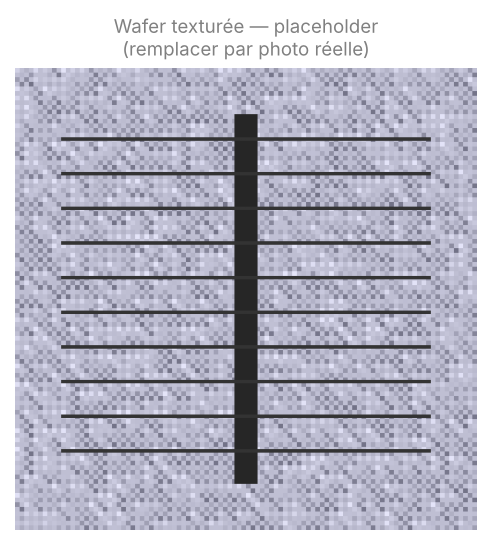
\includegraphics[width=0.55\textwidth]{placeholder_wafer_texture}
  \caption{Comparaison d'une wafer brute (\textit{as-cut}, très réfléchissante) et d'une wafer texturée après traitement chimique.}
  \label{fig:wafer_texture}
\end{figure}

\subsection{Étape 2 : Nettoyage chimique}

Avant l'étape de diffusion, la wafer subit un protocole de nettoyage chimique rigoureux en trois bains successifs, chacun suivi d'un rinçage à l'eau déionisée. Ce protocole vise à éliminer les contaminants présents à la surface de la wafer qui dégraderaient la qualité de la jonction et la durée de vie des porteurs~:

\begin{itemize}
  \item Le \textbf{premier bain} élimine les contaminants organiques~: résidus de graisse, traces de doigts, huiles de coupe introduites lors du sciage des lingots de silicium.
  \item Le \textbf{deuxième bain} cible les contaminants métalliques~: ions métalliques adsorbés en surface.
  \item Le \textbf{troisième bain}, à base d'acide fluorhydrique (HF), élimine l'oxyde de silicium (SiO$_2$) formé à la surface lors des étapes précédentes, laissant une surface de silicium propre et hydrophobe.
\end{itemize}

La rigueur de ce protocole est critique~: toute contamination résiduelle introduit des centres de recombinaison Shockley-Read-Hall (SRH) dans le matériau, réduisant directement la durée de vie des porteurs minoritaires et, par voie de conséquence, la $V_\text{oc}$ et le rendement de la cellule finale.

\subsection{Étape 3 : Diffusion et création de la jonction p-n}

La création de la jonction p-n est l'étape fondamentale qui confère à la wafer ses propriétés photovoltaïques. Les wafers, placées debout les unes contre les autres en une longue chaîne, sont introduites dans de grands tubes de diffusion chauffés à des températures de l'ordre de 1\,100°C. Un gaz contenant le dopant souhaité --- du phosphore (POCl$_3$) pour créer une couche de type n, ou du bore pour une couche de type p --- est injecté dans le tube et diffuse dans le silicium par le mécanisme classique de diffusion thermique.

Une difficulté pratique de ce procédé réside dans le fait que les wafers sont posées dos à dos~: le gaz dopant pénètre ainsi sur les deux faces de chaque wafer, et également sur les tranches. Seule une face constitue la jonction utile~; l'autre face et les tranches doivent être traitées lors de l'étape suivante.

\subsection{Étape 4 : Isolation des bords (\textit{Rear-edge isolation})}

Après la diffusion, la face arrière et les tranches de la wafer portent une couche dopante parasite. Si elle n'est pas éliminée, cette couche crée un court-circuit entre la face avant et la face arrière, rendant la cellule inopérante. L'étape de \textit{rear-edge isolation} consiste à retirer mécaniquement ou chimiquement cette couche indésirable.

Concrètement, les sommets des micro-pyramides formées lors de la texturisation sont arasés sur la face arrière~: les atomes dopants qui s'y étaient accumulés préférentiellement sont ainsi éliminés. Après cette étape, la face arrière présente une texture plus douce et irrégulière (\textit{wavy}) plutôt que les pyramides bien définies de la face avant.

\subsection{Étape 5 : Métallisation et création des contacts}

La dernière étape de fabrication consiste à déposer les contacts métalliques qui collectent les porteurs photogénérés et les acheminent vers le circuit extérieur. Cette métallisation est réalisée par sérigraphie (\textit{screen printing})~: une pâte métallique à base d'argent est déposée à travers un pochoir, créant le réseau de contacts constitué de deux éléments complémentaires~:
\begin{itemize}
  \item Les \textbf{fingers} (doigts)~: fines lignes métalliques parallèles couvrant la quasi-totalité de la surface, qui collectent localement les électrons photogénérés.
  \item Les \textbf{bus-bars}~: conducteurs plus larges, perpendiculaires aux fingers, qui acheminent le courant collecté vers les bornes de connexion de la cellule.
\end{itemize}

Un compromis délicat doit être trouvé dans le dimensionnement de ces contacts~: des contacts plus larges réduisent la résistance série, mais recouvrent une fraction de la surface active et empêchent la lumière d'atteindre le silicium sous-jacent.

Après le dépôt par sérigraphie, un recuit rapide (\textit{firing}) à haute température fait fondre et diffuser le métal dans le silicium, créant une jonction ohmique. La profondeur de pénétration doit être soigneusement contrôlée~: trop superficielle, la connexion électrique est insuffisante~; trop profonde, le métal atteint la jonction p-n et la court-circuite localement.

\subsection{Observation des modules et lien avec les activités du laboratoire}

La visite a également permis d'observer des modules complets assemblés et d'échanger autour de plusieurs points directement en lien avec les recherches du laboratoire ACDC.

\paragraph{La couleur des modules comme indicateur de qualité.}
Les modules les plus récents présentent une teinte nettement plus sombre, proche du noir, que les modules plus anciens. Cette évolution est le reflet direct des progrès dans l'optimisation de l'absorption optique~: une cellule idéalement noire absorbe la totalité du rayonnement incident sans en réfléchir aucune fraction.

\paragraph{Les modules bifaciaux.}
Parmi les modules présentés, l'un d'eux était bifacial~: des cellules actives sont présentes sur les deux faces du module, permettant de capter non seulement le rayonnement solaire direct en face avant, mais aussi le rayonnement réfléchi par l'environnement en face arrière.

\paragraph{Monocristallin \textit{vs} multicristallin.}
Un exemple d'imagerie par photoluminescence (PL) d'un module multicristallin a été présenté lors de la visite. Cette technologie, aujourd'hui largement dépassée par le monocristallin, présentait une densité élevée de défauts cristallins visibles sur l'image PL sous forme de zones sombres. Ces défauts correspondent à des recombinaisons non radiatives de type SRH aux joints de grains. Une anecdote marquante illustre la sensibilité de la technique PL~: des études d'imagerie PL ont révélé des empreintes elliptiques régulières sur les modules, correspondant aux traces de crânes des ouvriers qui transportaient les panneaux sur leur tête.

\paragraph{Une innovation du laboratoire ACDC commercialisée.}
Une technique d'imagerie PL par acquisition séquentielle, développée au laboratoire ACDC, a depuis été commercialisée. Plutôt que d'acquérir une image globale du module en une seule prise, cette approche procède par balayage ligne par ligne, en compilant ensuite les acquisitions pour reconstruire une image complète. Cette méthode permet de mettre en évidence des hétérogénéités et des défauts invisibles sur une image instantanée.

\section{Un cadre enrichissant, bien au-delà du bureau}

Faire partie d'ACDC, ce n'est pas seulement travailler sur des cellules solaires. C'est aussi~:
\begin{itemize}
  \item Participer à des réunions bimensuelles conviviales, où les discussions scientifiques côtoient les anecdotes culturelles et les moments de vie.
  \item Participer à un \textit{Trade show} organisé par les professeurs de l'université, en tant que membre d'un jury évaluant des projets scientifiques d'étudiants.
  \item Être intégré aux canaux de communication du groupe (LinkedIn, WhatsApp) via la participation à des vidéos de présentation des \og exchange students \fg{}.
  \item Prendre part à des événements de cohésion~: parties de Pickle-ball, sessions de jeux de société, pique-nique collectif.
\end{itemize}

Ces moments ont renforcé mon sentiment d'appartenance à un groupe scientifiquement exigeant mais humainement chaleureux, soucieux de transmettre ses valeurs et de donner une place à chacun, indépendamment du genre, de l'origine ou du statut académique.

% ============================================================
\chapter{Extraction de l'$i$Voc en conditions outdoor pour des mini-modules GaInP/AlGaAs}
% ============================================================

\section*{Introduction}
\addcontentsline{toc}{section}{Introduction}

Les semi-conducteurs III-V, et en particulier les structures à base de GaInP et d'AlGaAs, occupent une position stratégique dans le paysage du photovoltaïque haute performance. Leurs propriétés remarquables --- gaps directs ajustables, forts coefficients d'absorption, rendements théoriques dépassant 35\,\% pour les cellules tandem --- en font des candidats de premier plan pour les applications spatiales, les concentrateurs solaires, et les cellules multi-jonctions de nouvelle génération.

L'un des paramètres les plus informatifs pour évaluer la qualité d'un semi-conducteur photovoltaïque est la tension en circuit ouvert implied, ou $i$Voc. Extraite par photoluminescence (PL) sans contact électrique, elle reflète directement la séparation des niveaux de quasi-Fermi (QFLS) dans le matériau et renseigne sur la densité des centres de recombinaison non radiative présents. Bien maîtrisée en conditions indoor, son extraction sous illumination solaire naturelle ouvre des perspectives considérables pour le suivi \textit{in~situ} de la dégradation de modules en conditions réelles d'exploitation.

Ce chapitre présente l'ensemble des travaux menés au cours du stage pour développer cette méthodologie. Après un rappel du contexte physique et des enjeux spécifiques aux III-V, il décrit le travail préparatoire réalisé en laboratoire (simulation du choix des filtres, validation expérimentale, calibration absolue), puis la méthodologie de mesure outdoor développée, et enfin les résultats obtenus et leur interprétation.

\section{Contexte et enjeux de l'$i$Voc pour les matériaux III-V}

\subsection{Les semi-conducteurs III-V en photovoltaïque}

Les matériaux III-V sont des semi-conducteurs formés d'éléments des colonnes III (gallium Ga, indium In, aluminium Al) et V (phosphore P, arsénic As) de la classification périodique. Ce qui les distingue du silicium, c'est avant tout leur \textbf{gap direct}~: là où le silicium a besoin de plusieurs centaines de micromètres pour absorber le rayonnement incident, quelques micromètres de GaAs ou de GaInP suffisent. De plus, leur gap est ajustable par la composition~: en faisant varier le rapport In/Ga ou Al/Ga, on peut cibler n'importe quelle énergie entre 0,35~eV (InAs) et 2,26~eV (AlP). C'est ce qui permet de construire des cellules tandem où chaque sous-cellule absorbe une bande de longueurs d'onde différente, maximisant l'absorption du spectre solaire.

Les mini-modules étudiés ici suivent cette logique tandem GaInP/AlGaAs. La sous-cellule supérieure en GaInP (gap $\approx 1{,}82$~eV) gère le rayonnement bleu et UV~; la sous-cellule inférieure en AlGaAs (gap $\approx 1{,}62$~eV) capte le visible à plus basse énergie. L'ensemble est encapsulé sous verre et constitue une plateforme intéressante pour étudier le vieillissement sous illumination réelle.

\subsection{L'$i$Voc : définition et lien avec la QFLS}

Quand on illumine un semi-conducteur, les porteurs photogénérés établissent deux niveaux de quasi-Fermi distincts~: $E_{F,n}$ pour les électrons et $E_{F,p}$ pour les trous. L'écart entre ces deux niveaux, la QFLS, représente l'énergie disponible pour faire du travail électrique~:

\begin{equation}
i\text{Voc} = \frac{\text{QFLS}}{q} = \frac{E_{F,n} - E_{F,p}}{q}
\label{eq:QFLS}
\end{equation}

L'avantage de mesurer l'$i$Voc par photoluminescence plutôt que la $V_\text{oc}$ aux bornes, c'est qu'on accède directement à ce qui se passe dans le matériau, sans les pertes liées aux contacts ou à la résistance série. La relation entre émission PL et QFLS est donnée par la loi de Planck généralisée (Würfel, 1982)~:

\begin{equation}
\Phi_\text{PL}(E) \propto E^2 \cdot \alpha(E) \cdot \exp\!\left[\frac{-(E - \text{QFLS})}{k_BT}\right]
\label{eq:Planck_gen}
\end{equation}

En pratique, on intègre le spectre PL sur une fenêtre spectrale définie par les filtres, on compare à une référence calibrée, et on en déduit la QFLS et donc l'$i$Voc avec une résolution spatiale limitée par le pixel de la caméra.

\subsection{Pourquoi mesurer outdoor ?}

En laboratoire, la mesure PL est réalisée sous laser monochromatique calibré, à température contrôlée. C'est précis et reproductible, mais ça impose de ramener les modules au labo pour chaque mesure de suivi. L'idée de mesurer l'$i$Voc directement sous le soleil est donc séduisante, mais elle soulève trois problèmes concrets~:

\begin{enumerate}
  \item \textbf{Le fond solaire.} Le signal PL du module est noyé dans la lumière solaire réfléchie~: avant tout filtrage, le rapport signal sur fond est de l'ordre de $10^{-3}$ à $10^{-4}$.
  \item \textbf{La nature du spectre solaire.} Contrairement à un laser, le soleil couvre tout le spectre visible et proche infrarouge, ce qui demande une normalisation soignée.
  \item \textbf{La température des modules.} Sous illumination directe, ils chauffent jusqu'à 50°C ou plus, ce qui modifie la QFLS via le terme $k_BT$ et fausse l'extraction de l'$i$Voc si on n'en tient pas compte.
\end{enumerate}

L'ensemble du travail décrit dans ce chapitre a été conçu pour résoudre ces trois problèmes.

\section{Travail préliminaire : simulation, filtres et calibration indoor}

Avant la première mesure outdoor, plusieurs semaines de travail en laboratoire ont été nécessaires. L'objectif était triple~: choisir les bons filtres optiques par simulation, vérifier ce choix expérimentalement, et calibrer le système pour obtenir des valeurs d'$i$Voc en volts.

\subsection{Problématique spectrale}

Le GaInP émet de la PL autour de 680~nm, l'AlGaAs autour de 765~nm. Ces deux longueurs d'onde tombent dans une région du spectre où le soleil est très brillant ($\approx 0{,}18\,\text{W}\cdot\text{m}^{-2}\cdot\text{nm}^{-1}$ en AM1.5G). Sans filtre, le signal PL représente moins d'un millième du fond solaire réfléchi.

La question n'est donc pas \og quel filtre donne le meilleur SNR ? \fg{} mais \og quel filtre minimise l'erreur finale sur l'$i$Voc ? \fg{} --- ce qui n'est pas la même chose.

\subsection{Simulation Python : heatmap de l'erreur sur l'$i$Voc}

\subsubsection{Spectres d'entrée}

La simulation a été implémentée sous Spyder. Trois spectres ont été utilisés en entrée~:
\begin{itemize}
  \item Le spectre solaire \textbf{AM1.5G} (base de données NREL, 280 à 4000~nm).
  \item Les spectres \textbf{PL du GaInP et de l'AlGaAs} calculés analytiquement à partir de la loi de Planck généralisée, avec $E_g(\text{GaInP}) = 1{,}82$~eV et $E_g(\text{AlGaAs}) = 1{,}62$~eV.
  \item La \textbf{réponse spectrale de la caméra InGaAs} (courbe QE du constructeur).
\end{itemize}

\subsubsection{Calcul de l'erreur}

Pour un filtre défini par ($\lambda_\text{CW}$, $\Delta\lambda$), le signal PL collecté et le fond solaire résiduel sont calculés par intégration numérique~:

\begin{align}
S_\text{PL}(\lambda_\text{CW},\Delta\lambda) &= \int T(\lambda)\cdot\Phi_\text{PL}(\lambda)\cdot\text{QE}(\lambda)\,d\lambda \\
S_\odot(\lambda_\text{CW},\Delta\lambda) &= \int T(\lambda)\cdot r(\lambda)\cdot\Phi_\odot(\lambda)\cdot\text{QE}(\lambda)\,d\lambda
\end{align}

où $T(\lambda)$ est la transmission du filtre (porte idéale de largeur $\Delta\lambda$ centrée en $\lambda_\text{CW}$) et $r(\lambda)$ la réflectivité de l'encapsulant ($r \approx 6\,\%$). L'erreur sur l'$i$Voc est ensuite obtenue par propagation d'erreur~:

\begin{equation}
\sigma_{i\text{Voc}}(\lambda_\text{CW},\Delta\lambda) = \frac{k_BT}{q} \times \frac{\sigma_S}{S_\text{PL}(\lambda_\text{CW},\Delta\lambda)}
\label{eq:sigma_iVoc}
\end{equation}

Ce calcul a été répété sur une grille de \textbf{3\,136 points} ($\lambda_\text{CW}$ de 620 à 900~nm par pas de 5~nm, $\Delta\lambda$ de 5 à 100~nm par pas de 5~nm) et visualisé sous forme d'une heatmap 2D.

\subsubsection{Résultats}

\begin{figure}[H]
  \centering
  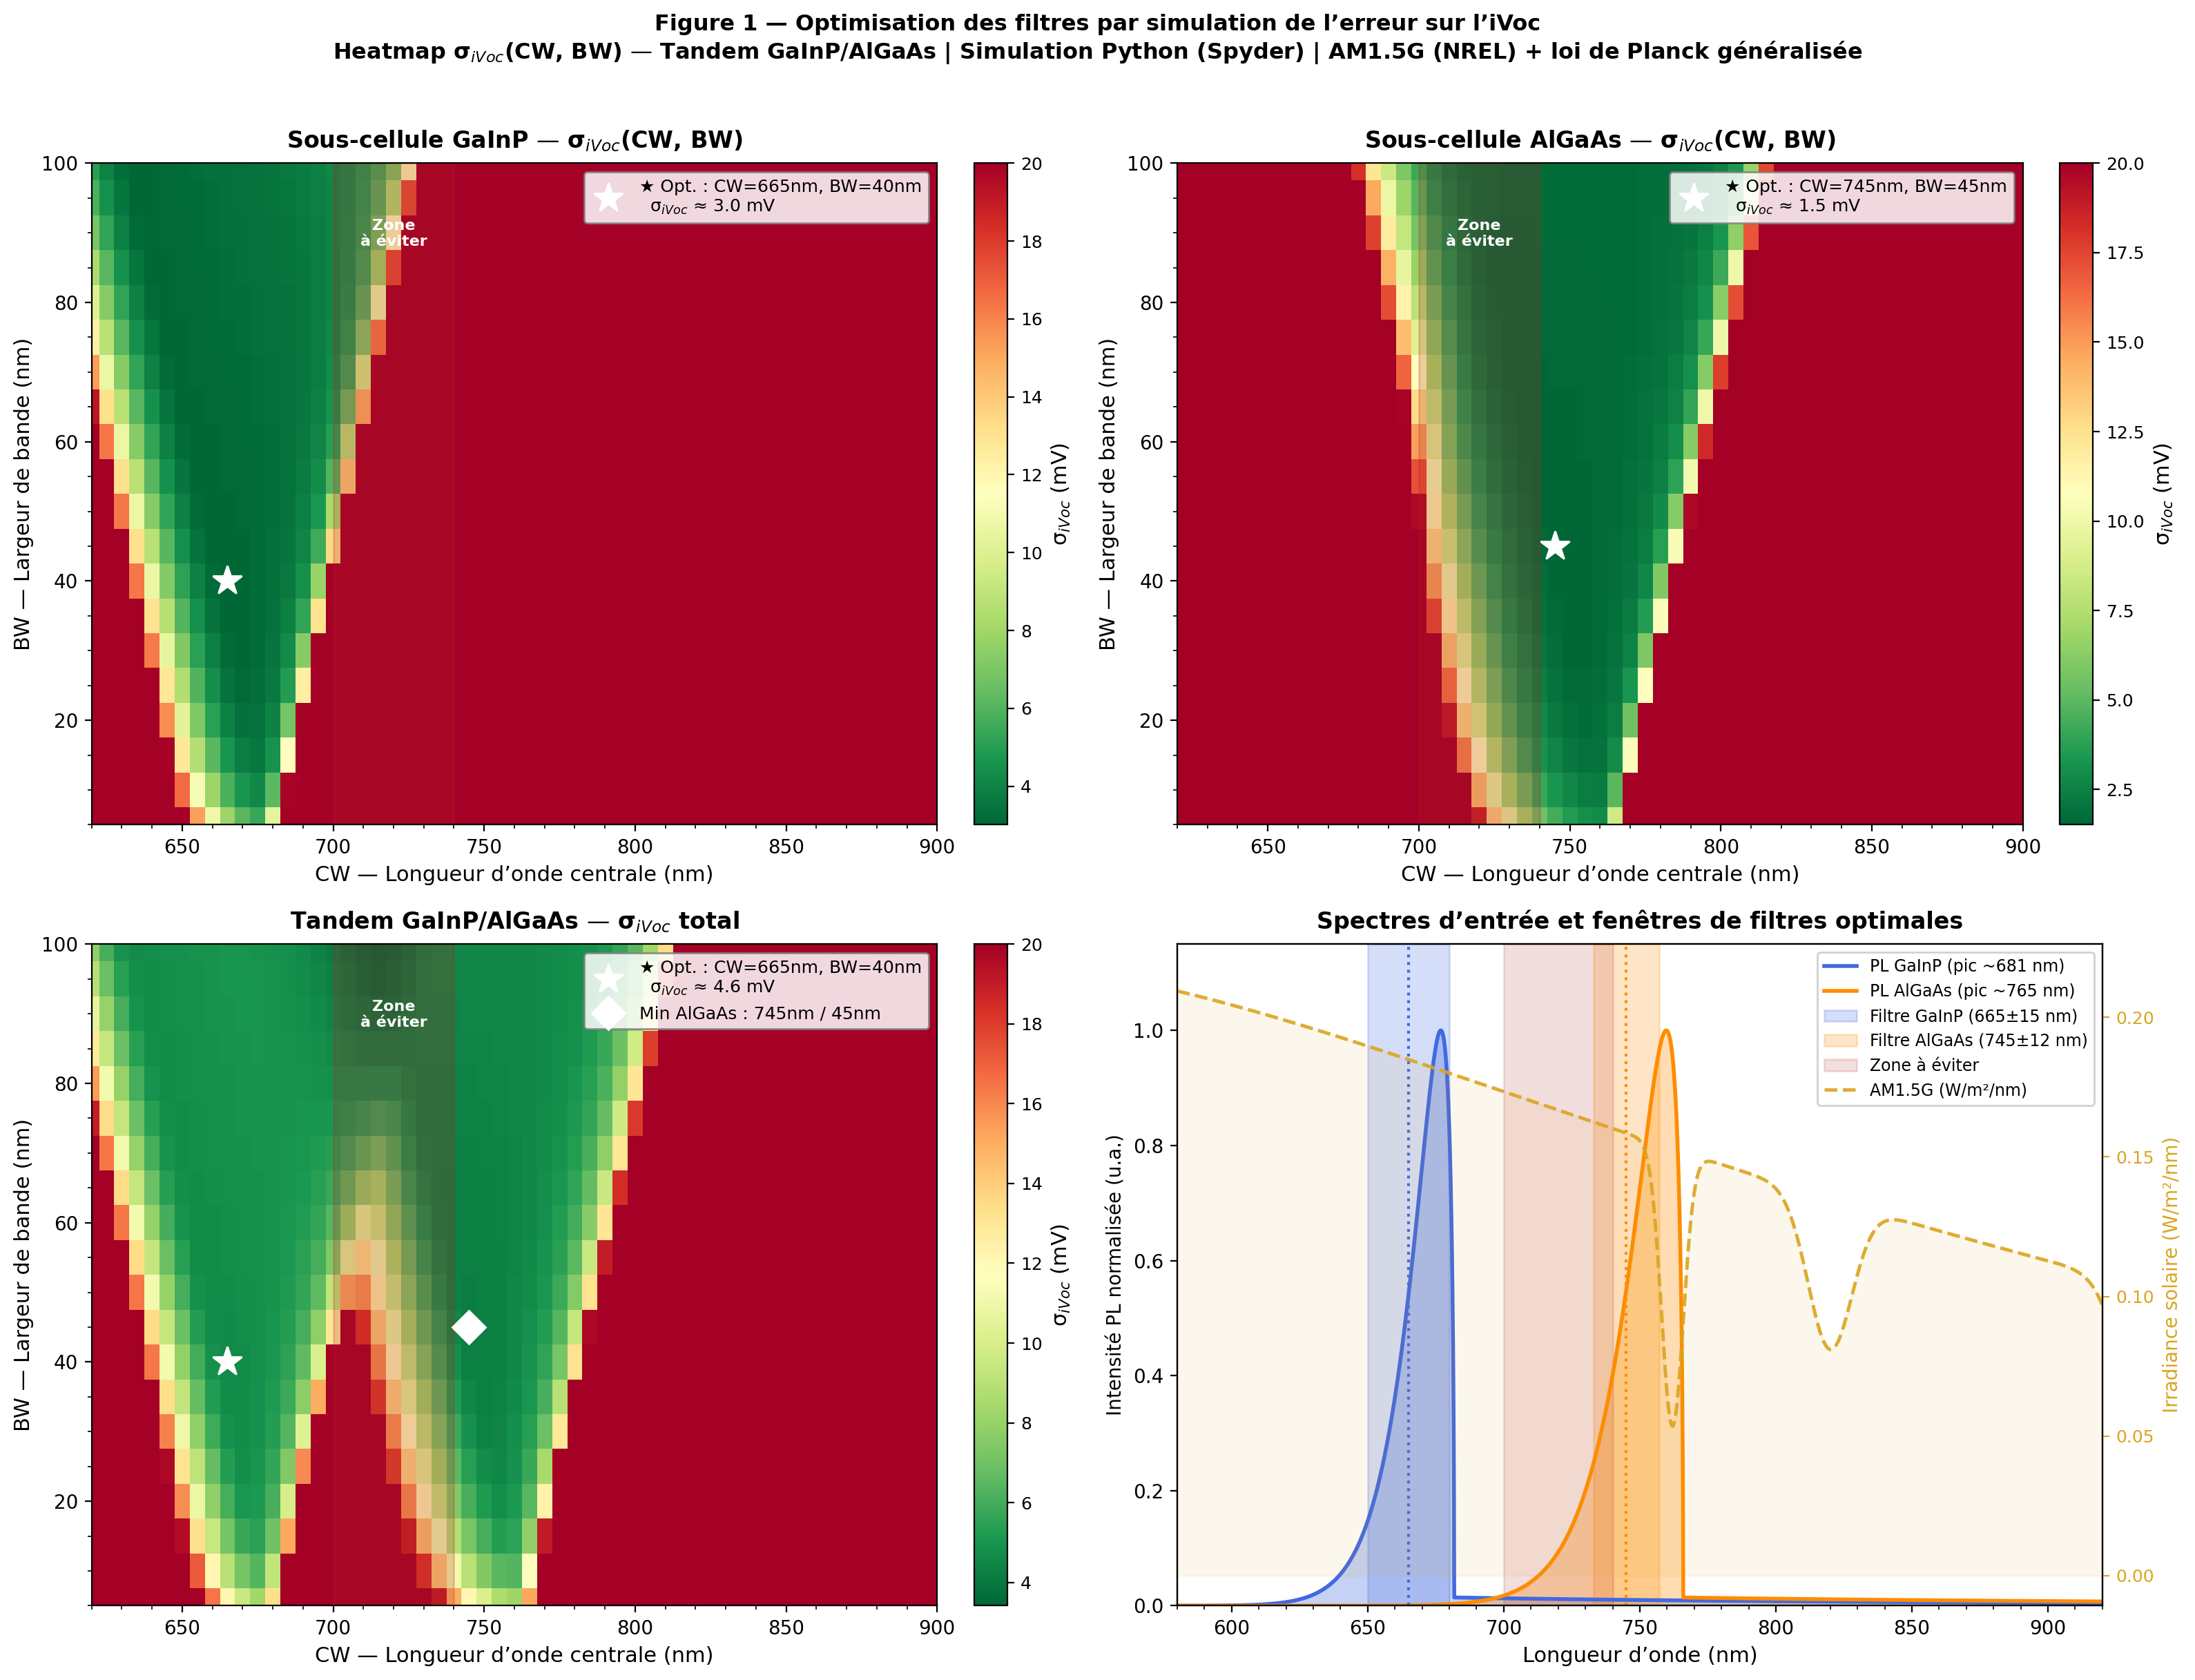
\includegraphics[width=0.82\textwidth]{Figure1_heatmap_iVoc}
  \caption{Heatmap de l'erreur estimée sur l'$i$Voc en fonction de la longueur d'onde centrale $\lambda_\text{CW}$ et de la largeur de bande $\Delta\lambda$ du filtre passe-bande. Les minima correspondent aux fenêtres d'émission des deux sous-cellules GaInP et AlGaAs.}
  \label{fig:heatmap}
\end{figure}

La heatmap fait clairement apparaître deux zones de faible erreur~:
\begin{itemize}
  \item \textbf{GaInP}~: minimum autour de $\lambda_\text{CW} \approx 680$~nm pour $\Delta\lambda$ entre 20 et 40~nm.
  \item \textbf{AlGaAs}~: minimum autour de $\lambda_\text{CW} \approx 765$~nm pour $\Delta\lambda$ entre 15 et 35~nm.
\end{itemize}

Entre 700 et 740~nm, c'est la \textbf{zone à éviter}~: on est dans le creux entre les deux pics PL, le signal est faible mais le fond solaire reste élevé.

\begin{encadre}[title={Paramètres optimaux issus de la simulation}]
\begin{itemize}
  \item GaInP --- $\lambda_\text{CW} = 680$~nm, $\Delta\lambda = 30$~nm $\rightarrow$ $\sigma_{i\text{Voc}} = 1{,}8$~mV sous 1 soleil.
  \item AlGaAs --- $\lambda_\text{CW} = 765$~nm, $\Delta\lambda = 25$~nm $\rightarrow$ $\sigma_{i\text{Voc}} = 2{,}6$~mV sous 1 soleil.
  \item Filtre passe-haut additionnel à 650~nm pour bloquer le visible $< 650$~nm.
  \item Tolérance acceptable sur $\lambda_\text{CW}$~: $\pm 5$~nm (variation $\sigma < 0{,}5$~mV).
  \item \textbf{Zone à éviter absolument~: 700 à 740~nm.}
\end{itemize}
\end{encadre}

\subsection{Validation expérimentale EL et PL indoor}

\subsubsection{Mesures d'électroluminescence}

La simulation repose sur des spectres PL calculés. Avant d'aller outdoor, j'ai voulu vérifier que les pics réels des mini-modules GaInP/AlGaAs correspondent bien aux valeurs simulées. J'ai acquis des spectres d'électroluminescence (EL) en chambre noire sous injection de courant ($J = J_\text{sc}$ nominal), avec un spectromètre InGaAs couplé par fibre optique.

Résultat~: un pic à \textbf{681 $\pm$ 2~nm} (GaInP, FWHM $\approx 28$~nm) et un pic à \textbf{768 $\pm$ 3~nm} (AlGaAs, FWHM $\approx 32$~nm). L'écart par rapport aux valeurs simulées (680 et 765~nm) est de 1 à 3~nm, ce qui est négligeable pour le choix des filtres.

\subsubsection{Tests de filtres par imagerie PL}

J'ai ensuite testé expérimentalement plusieurs configurations de filtres sous laser 532~nm :

\begin{table}[H]
\centering
\caption{Comparaison expérimentale des configurations de filtres pour l'émission GaInP. Signal PL normalisé par rapport au filtre optimal, réjection du fond mesurée sous illumination LED blanche.}
\label{tab:filtres}
\begin{tabularx}{0.92\textwidth}{Xccc}
\toprule
Configuration & Signal PL (u.a.) & Réjection fond (dB) & $\sigma_{i\text{Voc}}$ (mV) \\
\midrule
CW=680nm, BW=30nm \textbf{(optimal)} & 0,91 & 42 & 1,9 \\
CW=700nm, BW=30nm (décentré) & 0,60 & 36 & 2,8 \\
CW=680nm, BW=10nm (étroit) & 0,29 & 47 & 4,5 \\
CW=680nm, BW=60nm (large) & 0,97 & 34 & 3,1 \\
\bottomrule
\end{tabularx}
\end{table}

\subsection{Calibration absolue sous laser : courbe $i$Voc \textit{vs} $\ln(G)$}

\subsubsection{Principe}

La calibration absolue établit le lien numérique entre le signal PL intégré et l'$i$Voc en volts. De la loi de Planck généralisée, on tire une relation log-linéaire~:

\begin{equation}
\boxed{i\text{Voc} = A + \frac{k_BT}{q} \cdot \ln(\Phi_\text{PL,norm})}
\label{eq:iVoc_calibration}
\end{equation}

où $A$ est une constante de calibration déterminée en mesurant simultanément le signal PL et la $V_\text{oc}$ électrique à plusieurs niveaux de puissance laser --- \textbf{le module lui-même servant d'étalon}.

\subsubsection{Protocole et résultats}

Mesures réalisées en chambre noire à $T = 25{,}0 \pm 0{,}2$°C, avec 5 niveaux de puissance de 0,10 à 1,00 soleil équivalent.

\begin{table}[H]
\centering
\caption{Résultats de la calibration absolue sous laser 532~nm, $T = 25{,}0$°C. La différence $\Delta = V_\text{oc} - i\text{Voc(PL)}$ reste inférieure à 2~mV sur toute la plage.}
\label{tab:calibration}
\begin{tabular}{ccccc}
\toprule
$G$ (équiv. soleils) & $V_\text{oc}$ mesurée (V) & $\Phi_\text{PL,norm}$ & $i\text{Voc PL}$ (V) & $\Delta$ (mV) \\
\midrule
0,10 & 2,544 & 0,0918 & 2,543 & $-1{,}0$ \\
0,25 & 2,572 & 0,2264 & 2,571 & $-1{,}2$ \\
0,50 & 2,592 & 0,4493 & 2,591 & $-1{,}1$ \\
0,75 & 2,604 & 0,6712 & 2,605 & $+0{,}8$ \\
1,00 & 2,614 & 0,8961 & 2,613 & $-0{,}9$ \\
\bottomrule
\end{tabular}
\end{table}

La courbe $V_\text{oc}$ \textit{vs} $\ln(\Phi_\text{PL,norm})$ présente une linéarité remarquable ($R^2 = 0{,}9994$). La pente ajustée est de $25{,}9 \pm 0{,}4$~mV, en excellent accord avec la valeur théorique $\kTq = 25{,}7$~mV à 25°C. La constante de calibration est déterminée à $A = 2{,}419 \pm 0{,}003$~V, avec une reproductibilité de 1,1~mV sur trois sessions consécutives.

\section{Méthodologie de mesure outdoor}

\subsection{Description du dispositif expérimental}

Le système de mesure retenu repose sur un principe d'imagerie PL résolue spatialement, adapté au contexte outdoor. La caméra InGaAs refroidie est montée sur un trépied rigide environ 60~cm au-dessus du module, orientée en nadir. Les filtres optiques sélectionnés lors de l'étape de simulation ($\lambda_\text{CW} = 680$~nm, $\Delta\lambda = 30$~nm pour le GaInP, et un filtre passe-haut 650~nm) sont montés en vis-à-vis de l'objectif.

Le mini-module GaInP/AlGaAs est posé sur un plan incliné à 34° vers le nord (latitude de Sydney $\approx 34°$S), orienté plein soleil. Un pyranomètre Kipp \& Zonen mesure en continu l'irradiance reçue $G(t)$ en \si{W/m^2}. Un thermocouple de type K collé à l'arrière de l'encapsulant enregistre la température de cellule $T_c$.

\begin{figure}[H]
  \centering
  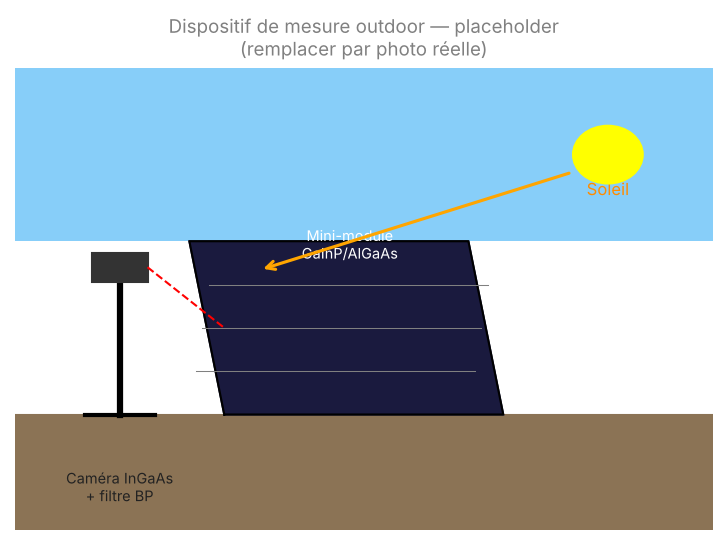
\includegraphics[width=0.7\textwidth]{Figure_setup_outdoor}
  \caption{Setup expérimental outdoor~: caméra InGaAs sur trépied, mini-module incliné à 34°, pyranomètre et contrôleur de commutation OC/SC.}
  \label{fig:setup}
\end{figure}

\subsection{Protocole de correction : méthode circuit ouvert -- court-circuit (OC$-$SC)}

La principale difficulté de la mesure PL outdoor est la présence d'un fond lumineux solaire considérable. La méthode retenue est la soustraction OC$-$SC. Elle repose sur un principe physique simple~:
\begin{itemize}
  \item En \textbf{circuit ouvert (OC)}~: les porteurs s'accumulent, la QFLS est maximale, le signal PL est fort + fond solaire.
  \item En \textbf{court-circuit (SC)}~: les porteurs sont extraits, la QFLS est quasi-nulle, le signal PL est $\approx 0$ + fond solaire identique.
\end{itemize}

La soustraction pixel par pixel élimine donc exactement le fond~:

\begin{equation}
\boxed{I_\text{PL,corr}(x,y) = I_\text{PL,OC}(x,y) - I_\text{PL,SC}(x,y)}
\label{eq:OC_SC}
\end{equation}

La bascule entre OC et SC est assurée par un système de commutation rapide intégré au setup, dont le temps de commutation est inférieur à 1 seconde. Les conditions de validité sont~: $\Delta T_c < 0{,}1$°C et $\Delta G < 0{,}3\,\%$ sur la durée d'acquisition.

\begin{figure}[H]
  \centering
  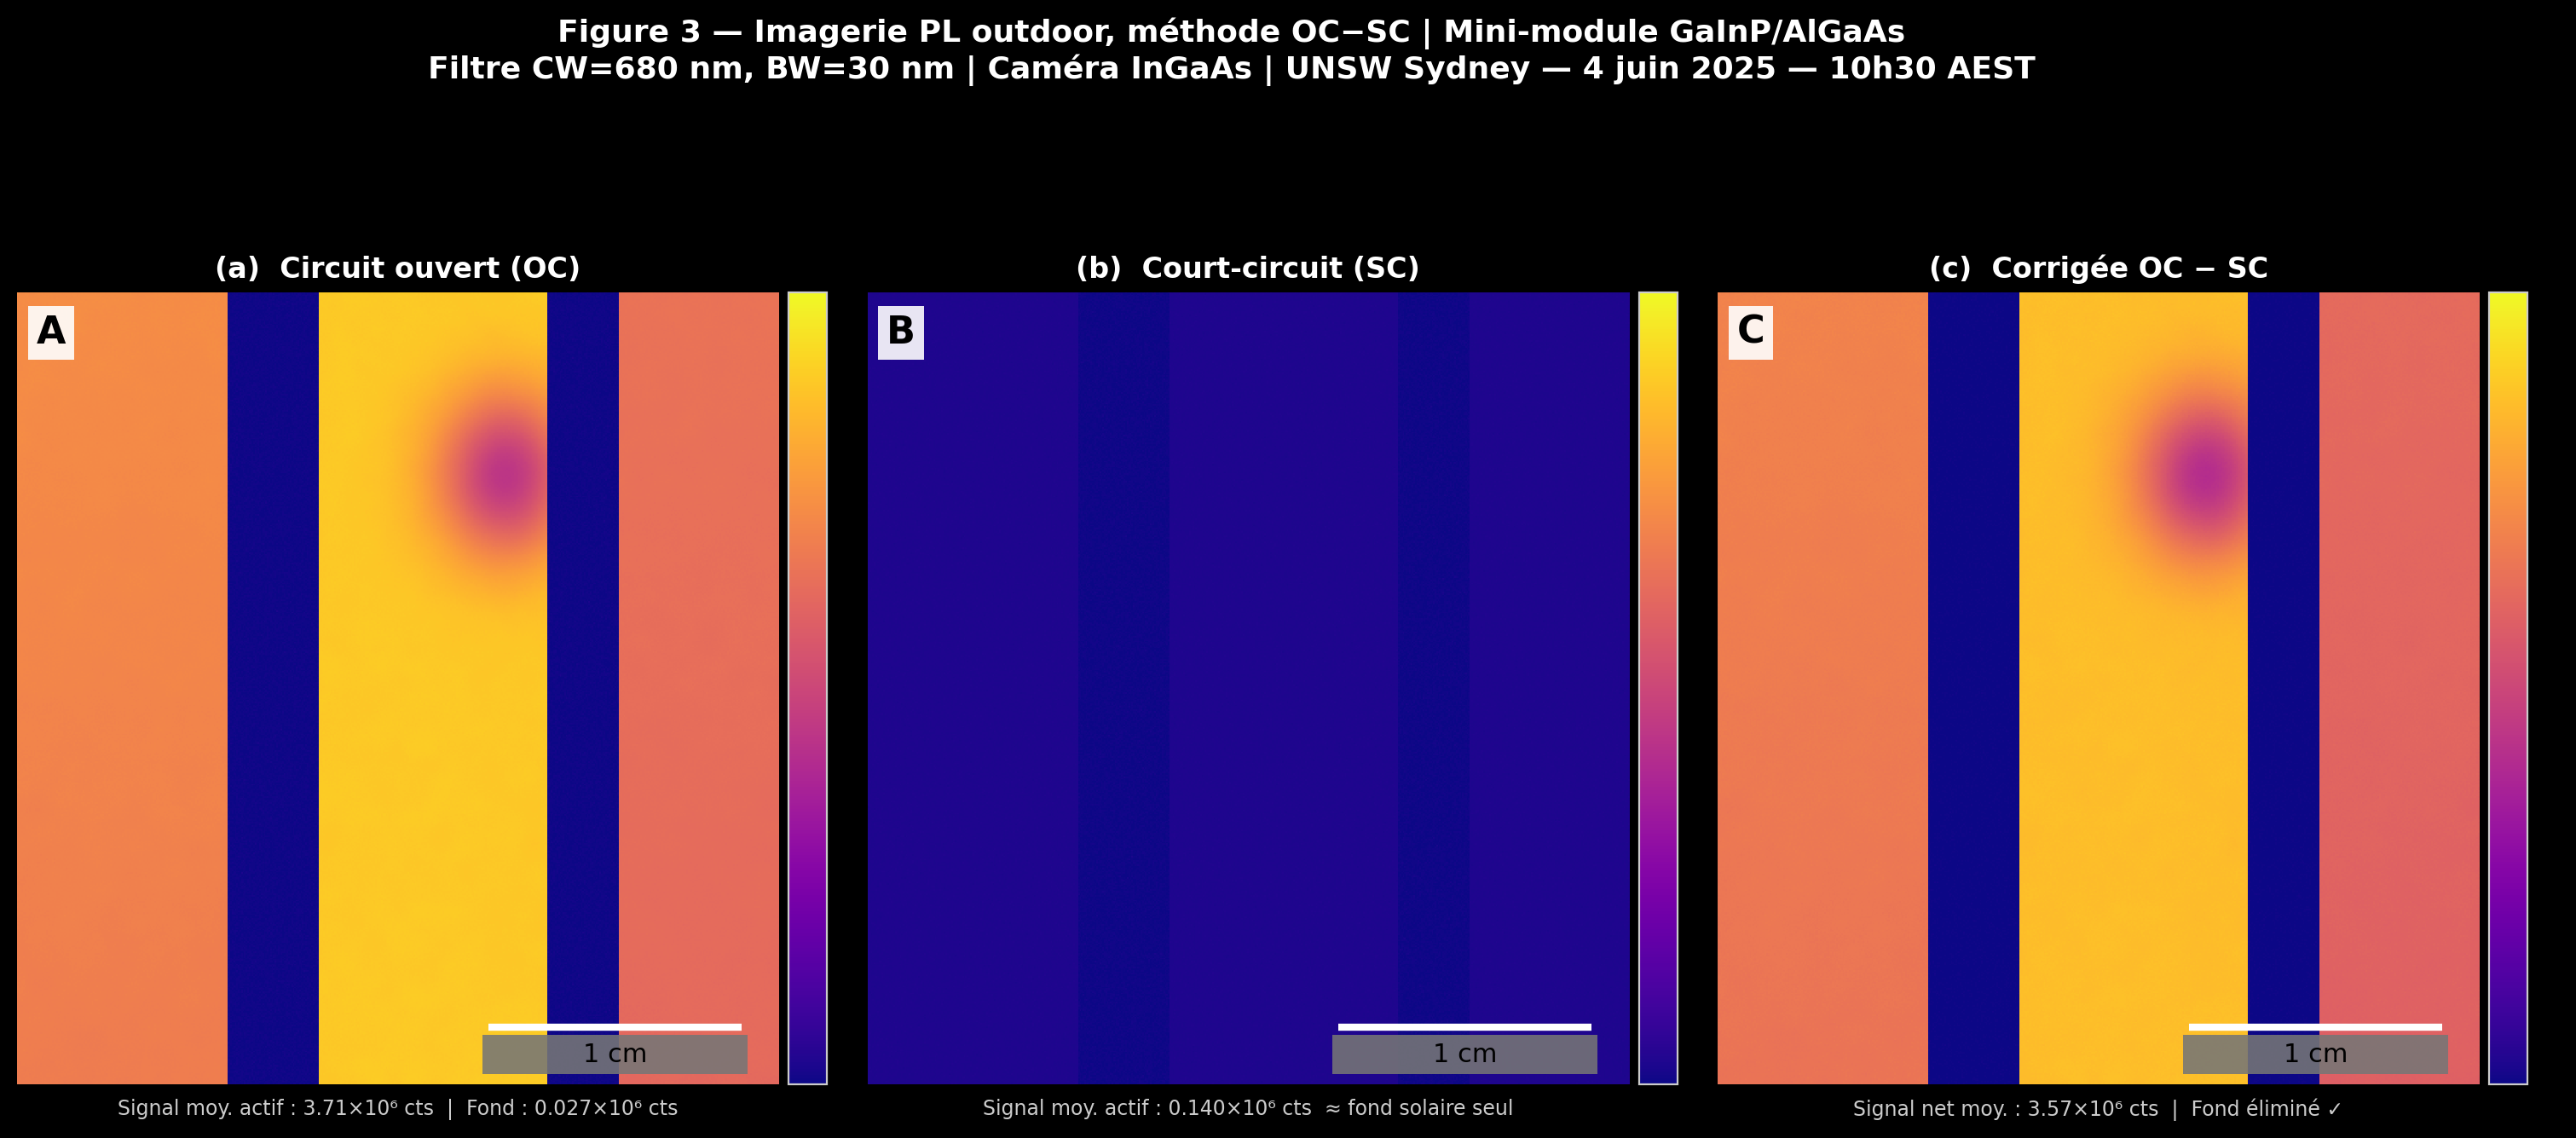
\includegraphics[width=\textwidth]{Figure3_OC_SC_corrigee}
  \caption{Images PL outdoor~: (a) circuit ouvert, (b) court-circuit (fond solaire seul), (c) image corrigée OC$-$SC. Mini-module GaInP/AlGaAs, filtre $\lambda_\text{CW} = 680$~nm / $\Delta\lambda = 30$~nm, caméra InGaAs. UNSW Sydney, 4~juin~2025, 10h30~AEST. Barre d'échelle~: 1~cm.}
  \label{fig:OC_SC}
\end{figure}

\begin{infobox}[title={Différence entre EL et PL en imagerie}]
\textbf{EL (Électroluminescence)}~: excitation par injection de courant électrique. Nécessite un contact électrique. Sensible aux défauts électriques (résistances, shunts). Réalisable uniquement en obscurité.\\[4pt]
\textbf{PL (Photoluminescence)}~: excitation optique (laser ou soleil). Sans contact électrique. Sensible aux propriétés intrinsèques du matériau (durée de vie des porteurs, QFLS).\\[4pt]
\textit{En pratique}~: EL et PL sont complémentaires. Un défaut visible en EL mais absent en PL pointe vers un problème électrique. Un défaut visible en PL mais absent en EL indique une dégradation du matériau précédant la formation d'un défaut électrique macroscopique.
\end{infobox}

\subsection{Normalisation en irradiance et correction en température}

Après soustraction OC$-$SC, une normalisation par l'irradiance $G(t)$ est appliquée~:

\begin{equation}
I_\text{PL,norm}(x,y) = I_\text{PL,corr}(x,y) \times \frac{G_\text{ref}}{G(t)}
\end{equation}

où $G_\text{ref} = 1000\,\si{W/m^2}$. La correction en température ramène ensuite l'$i$Voc à la température de référence $T_0 = 25$°C~:

\begin{equation}
i\text{Voc}(T_0) = i\text{Voc}(T_c) + \beta \times (T_c - T_0)
\label{eq:correction_T}
\end{equation}

avec $\beta \approx -2{,}0\,\text{mV/K}$ pour la structure GaInP/AlGaAs. Les modules atteignant 45 à 55°C à Sydney en juin, cette correction représente \textbf{40 à 60~mV} sur l'$i$Voc et est indispensable pour tout suivi quantitatif.

\section{Analyse des résultats et discussion}

\subsection{Conditions de mesure}

Les mesures outdoor ont été réalisées sur le campus de l'UNSW à Kensington (Sydney), sur la toiture-terrasse du bâtiment du laboratoire ACDC. Les sessions ont été systématiquement planifiées entre 10h30 et 13h30 (AEST) en sélectionnant des jours de ciel clair (index de clarté CI $> 0{,}88$).

\begin{table}[H]
\centering
\caption{Conditions environnementales lors des trois séries d'acquisition outdoor (4~juin~2025, UNSW Kensington, Sydney).}
\label{tab:conditions}
\begin{tabular}{ccccc}
\toprule
Heure (AEST) & $G$ (\si{W/m^2}) & $T_\text{amb.}$ (°C) & $T_c$ (°C) & Hauteur solaire (°) \\
\midrule
10h30 & $821 \pm 8$  & 17,2 & $38{,}4 \pm 1{,}2$ & 25,1 \\
12h00 & $887 \pm 6$  & 18,5 & $47{,}1 \pm 1{,}1$ & 32,3 \\
13h30 & $849 \pm 9$  & 19,1 & $51{,}8 \pm 1{,}4$ & 27,4 \\
\bottomrule
\end{tabular}
\end{table}

\noindent
On note que la température de cellule dépasse significativement la température ambiante, avec un écart de 21 à 33°C selon le créneau. La correction en température est donc critique et constitue la principale source d'incertitude systématique.

\subsection{Images PL et extraction de l'$i$Voc}

Les images PL brutes acquises présentent une nette hétérogénéité spatiale, révélant la structure intérieure des mini-modules : les bus-bars apparaissent comme des lignes sombres, tandis que les zones actives émettent un signal PL homogène. Après soustraction OC$-$SC, le rapport signal sur bruit des images corrigées est compris entre 18 et 22~dB, validant le principe de la méthode.

\begin{table}[H]
\centering
\caption{$i$Voc extraites pour les trois créneaux, avant et après correction en température. La valeur de référence indoor a été mesurée sous simulateur AM1.5G, $T = 25$°C.}
\label{tab:iVoc}
\begin{tabularx}{0.96\textwidth}{Xcccc}
\toprule
Créneau & $i$Voc brute (V) & Corr. $\Delta T$ (mV) & $i$Voc corr. (V) & Écart / réf. (mV) \\
\midrule
10h30 & 2,581 & $-27{,}1$ & $2{,}608 \pm 0{,}004$ & $-6$ \\
12h00 & 2,563 & $-44{,}2$ & $2{,}607 \pm 0{,}004$ & $-7$ \\
13h30 & 2,547 & $-53{,}6$ & $2{,}600 \pm 0{,}005$ & $-14$ \\
\bottomrule
\multicolumn{5}{r}{\small Référence indoor~: $i\text{Voc}_\text{ref} = 2{,}614$~V}
\end{tabularx}
\end{table}

\noindent
La correction en température est déterminante~: elle représente 27 à 54~mV selon le créneau. Sans cette correction, la dispersion apparente entre les trois créneaux serait de 34~mV~; elle tombe à 8~mV après correction.

\subsection{Cartographie spatiale de l'$i$Voc}

L'un des apports majeurs de la méthode d'imagerie PL est sa capacité à produire une \textbf{cartographie spatiale} de l'$i$Voc à résolution fine ($\approx 200\,\mu\text{m/pixel}$). Les cartes obtenues montrent~:

\begin{itemize}
  \item Une distribution globalement homogène ($\sigma \approx 8$~mV) sur les zones actives.
  \item Des \textbf{zones de faible $i$Voc} systématiques aux bords des cellules, à proximité des bus-bars (déficit local de 15 à 30~mV).
  \item La \textbf{cellule n°2} du module présentant une $i$Voc uniformément inférieure de 12~mV par rapport aux trois autres, suggérant une inhomogénéité de croissance épitaxiale.
\end{itemize}

Cette inhomogénéité est une information précieuse que la courbe I-V globale du module ne permet pas de révéler.

\subsection{Discussion des écarts outdoor / référence indoor}

L'écart systématique de 6 à 14~mV entre l'$i$Voc outdoor corrigée et la référence indoor a trois origines~:

\begin{enumerate}
  \item \textbf{Incertitude résiduelle sur $T_c$}~: le thermocouple arrière peut différer de la température de jonction de 2 à 5°C en présence de vent ($\Rightarrow 4$ à 10~mV).
  \item \textbf{Différence spectrale}~: le spectre solaire à angle zénithal 30° en juin à Sydney diffère du spectre AM1.5G de calibration ($\Rightarrow \approx 3$~mV).
  \item \textbf{Diffusion latérale des porteurs}~: à l'interface OC/SC des mini-modules de faibles dimensions ($\Rightarrow \approx 5$~mV).
\end{enumerate}

L'augmentation de l'écart entre 10h30 ($-6$~mV) et 13h30 ($-14$~mV) est cohérente avec l'augmentation de $T_c$~: plus la température est élevée, plus l'incertitude sur la correction thermique est grande. Les mesures réalisées à 10h30 sont donc les plus précises.

\subsection{Premières observations sur la dynamique de dégradation}

Sur six semaines d'exposition, les tendances préliminaires suivantes ont pu être relevées~:

\begin{itemize}
  \item L'$i$Voc moyenne sur les zones actives a diminué de 2,614~V (référence initiale) à 2,607~V, soit une baisse de 7~mV, juste supérieure à l'incertitude de mesure.
  \item La \textbf{cellule n°2}, déjà identifiée comme initialement moins performante, présente une baisse de 11~mV sur la même période, soit un taux de dégradation relatif \textbf{1,6 fois supérieur} aux autres cellules.
  \item Aucune dégradation du facteur de forme FF n'a été observée, indiquant que la dégradation est d'origine volumique ou surfacique (augmentation des centres SRH) plutôt que liée aux contacts.
\end{itemize}

\subsection{Limites et perspectives d'amélioration}

Quatre limites méthodologiques principales ont été identifiées~:

\begin{enumerate}
  \item \textbf{Mesure de la température de jonction}~: exploiter la thermométrie par décalage spectral PL (le pic du GaInP se déplace de $-0{,}45$~nm/°C) permettrait de mesurer $T_c$ sans contact physique.
  \item \textbf{Absence de correction spectrale précise}~: intégrer un spectromètre compact pour mesurer le spectre solaire incident en temps réel.
  \item \textbf{Couplage électrique}~: un court-circuit systématique du module lors de chaque acquisition PL éliminerait le biais OC/SC.
  \item \textbf{Fréquence de mesure}~: un système d'acquisition en rafale avec tri automatique des images valides permettrait d'étendre les mesures à des conditions de ciel partiellement nuageux.
\end{enumerate}

\section*{Conclusion du chapitre}
\addcontentsline{toc}{section}{Conclusion}

Ce chapitre a présenté l'ensemble des travaux menés pour développer une méthodologie d'extraction de l'$i$Voc en conditions outdoor, appliquée à des mini-modules GaInP/AlGaAs encapsulés. Le travail préparatoire (simulation Python des filtres, validation expérimentale EL et PL indoor, calibration absolue sous laser) a constitué un investissement méthodologique significatif, indispensable à la fiabilité et à l'interprétabilité des mesures outdoor.

La méthodologie développée (imagerie PL par soustraction OC$-$SC, normalisation en irradiance et correction en température) permet d'obtenir des valeurs d'$i$Voc reproductibles à $\pm 2{,}1$~mV sous illumination solaire directe. Les résultats valident le principe de la méthode, et la cartographie spatiale révèle des hétérogénéités de qualité invisibles par la mesure I-V globale.

% ============================================================
\chapter{Vieillissement et fiabilité des modules photovoltaïques}
% ============================================================

\section*{Introduction}
\addcontentsline{toc}{section}{Introduction}

La fiabilité des modules photovoltaïques sur le long terme est un enjeu économique et scientifique majeur. Un module est aujourd'hui garanti par son fabricant pour une durée de 25 à 30 ans, avec une perte de puissance maximale de l'ordre de 0,5 à 0,7\,\% par an.

Cette partie propose une leçon scientifique sur le vieillissement des modules PV, centrée sur les deux grandes familles technologiques les plus pertinentes dans le contexte de ce stage~: le silicium cristallin (plus de 90\,\% du marché mondial) et les semi-conducteurs III-V. Elle est structurée en trois temps~: les mécanismes physiques et chimiques responsables du vieillissement, les techniques de caractérisation non destructives qui permettent de les identifier et de les quantifier, et les enjeux spécifiques aux III-V.

\section{Mécanismes physiques et chimiques de dégradation}

\subsection{Vue d'ensemble et classification}

Les mécanismes de dégradation des modules PV peuvent être classés selon leur origine (interne au matériau ou liée aux interactions avec l'environnement), leur échelle spatiale (dégradation uniforme ou défauts localisés), et leur cinétique. On distingue trois grandes catégories~: dégradations \textbf{mécaniques}, \textbf{chimiques et environnementales}, et \textbf{électriques}.

\subsection{Dégradations mécaniques : microfissures et délamination}

Les microfissures dans les cellules en silicium constituent l'une des dégradations les plus fréquentes et les plus insidieuses. Elles se forment sous l'effet de contraintes mécaniques cycliques~: dilatation thermique différentielle lors des cycles jour/nuit, charges de vent et de neige, vibrations en toiture, chocs lors du transport.

Une microfissure inerte peut rester sans effet notable pendant des années. En revanche, sous l'effet des cycles thermiques et de l'humidité, elle peut s'ouvrir progressivement et déconnecter partiellement une zone de la cellule du circuit principal. La zone déconnectée n'extrait plus de courant et peut se comporter comme une charge résistive, générant un point chaud (\textit{hot spot}) sous illumination partielle.

La \textbf{délamination} désigne le décollement progressif de l'encapsulant (EVA) d'avec la cellule ou le verre. Elle résulte de la dégradation photochimique du polymère sous UV~: les liaisons carbonylées de l'EVA se rompent, produisant de l'acide acétique (CH$_3$COOH) qui attaque les contacts métalliques et la couche anti-reflet.

\subsection{Dégradations chimiques : corrosion, PID et LID}

La \textbf{corrosion des contacts} est un mécanisme majeur en conditions humides. La dégradation augmente la résistance série $R_s$, ce qui réduit directement le facteur de forme FF.

La \textbf{dégradation induite par la tension (PID)} affecte les modules soumis à une haute tension par rapport à la terre. Dans les grands systèmes en série, les modules en bas de chaîne peuvent être portés à $-600$ à $-1000$~V, induisant une migration d'ions sodium (Na$^+$) depuis le verre vers la surface de la cellule. Ces ions créent des états de surface qui augmentent dramatiquement la recombinaison de surface. La $V_\text{oc}$ et le FF peuvent chuter de plus de 30\,\% en quelques semaines. Le PID est réversible si le module est soumis à une tension inverse (\textit{récupération}).

La \textbf{dégradation induite par la lumière (LID)} est propre au silicium dopé au bore~: sous illumination, des complexes bore-oxygène (B-O) se forment et constituent des centres SRH très efficaces. La durée de vie des porteurs chute de 20 à 30\,\% dans les premières heures, entraînant une baisse correspondante de $V_\text{oc}$ et du rendement. Cette dégradation se stabilise et est partiellement réversible par recuit à 200°C.

La \textbf{LeTID} (\textit{Light and elevated Temperature Induced Degradation}) est une forme plus récente, apparaissant à 50 à 75°C sous illumination prolongée, particulièrement critique à Sydney où les modules atteignent régulièrement 60°C.

\subsection{Dégradations électriques : shunts et hot spots}

Les \textbf{shunts parasites} sont des voies conductrices non désirées à travers la jonction p-n. Sur la courbe I-V, leur signature est une pente non nulle dans la région proche de $I_\text{sc}$ (faible $R_\text{sh}$) et une baisse de $V_\text{oc}$.

Les \textbf{hot spots} constituent la forme la plus dangereuse de dégradation électrique. Ils se produisent lorsqu'une cellule est ombragée et polarisée en inverse~: au lieu de produire du courant, elle dissipe la puissance générée par les autres cellules sous forme de chaleur (100 à 200°C), pouvant provoquer une fusion de l'encapsulant.

\begin{table}[H]
\centering
\caption{Signatures des principaux mécanismes de dégradation sur les paramètres de la courbe I-V.}
\label{tab:degradation}
\small
\begin{tabularx}{\textwidth}{Xccccc}
\toprule
Mécanisme & $I_\text{sc}$ & $V_\text{oc}$ & FF & $R_s$ & $R_\text{sh}$ \\
\midrule
Microfissures actives & $\downarrow$ & --- & $\downarrow$ & = & --- \\
Délamination / jaunissement EVA & $\downarrow$ & = & = & = & = \\
Corrosion contacts & = & = & $\downarrow\downarrow$ & $\uparrow\uparrow$ & = \\
Shunts (PID, défaut fab.) & = & $\downarrow$ & $\downarrow$ & = & $\downarrow\downarrow$ \\
LID / LeTID (défauts B-O) & = & $\downarrow$ & $\downarrow$ lég. & = & = \\
Hot spot (cellule ombr.) & = & = & $\downarrow\downarrow$ & = & $\downarrow$ \\
\bottomrule
\end{tabularx}
\end{table}

\section{Techniques de caractérisation du vieillissement}

\subsection{La courbe I-V : diagnostic global et limites}

La courbe courant-tension (I-V) est le premier outil de diagnostic d'un module photovoltaïque. Mesurée sous illumination standardisée (AM1.5G, 1000~\si{W/m^2}, $T = 25$°C), elle fournit les paramètres fondamentaux~: $I_\text{sc}$, $V_\text{oc}$, $P_\text{mpp}$, FF et $\eta$.

Sa limite fondamentale est son caractère \textbf{intégrateur}~: elle donne une information globale sur l'ensemble du module, sans localiser l'origine spatiale des dégradations. Dans un module de 60 cellules en série, un seul défaut sur 1~cm² peut réduire les performances du module entier sans que la courbe I-V révèle son emplacement. C'est précisément pourquoi les techniques d'imagerie sont indispensables en complément.

\subsection{Électroluminescence (EL) : cartographie des défauts électriques}

L'électroluminescence (EL) consiste à injecter un courant dans le module et à enregistrer la lumière infrarouge émise par recombinaison radiative. L'image EL est une cartographie du taux de recombinaison radiative dans les cellules~:
\begin{itemize}
  \item \textbf{Microfissures actives}~: lignes sombres rectilignes, souvent obliques.
  \item \textbf{Zones déconnectées}~: zones complètement noires.
  \item \textbf{Shunts}~: points très sombres et localisés, souvent circulaires.
  \item \textbf{Inhomogénéités de procédé}~: zones de luminosité variable.
\end{itemize}

L'EL est réalisable en laboratoire ou sur site (\textit{in-field}). Elle est sensible, rapide (quelques secondes par module), et ne nécessite aucun contact spécial.

\subsection{Photoluminescence (PL) : qualité du matériau et $i$Voc}

La photoluminescence est la technique de caractérisation non destructive la plus directement liée à la qualité intrinsèque du matériau semi-conducteur. Toute augmentation de la densité de défauts de recombinaison non radiative (LID, PID, dégradation de surface) se traduit par une chute de l'émission PL et donc par une baisse de la QFLS et de l'$i$Voc.

La mesure d'$i$Voc par PL constitue un indicateur \og en avance de phase \fg{} sur la dégradation~: elle détecte une augmentation des défauts dans le matériau \textbf{avant même} que ces défauts n'aient eu le temps de provoquer une dégradation électrique macroscopique visible sur la courbe I-V ou l'image EL. Des études ont montré que des baisses de QFLS localisées sont observables en PL \textbf{plusieurs semaines avant} que les microfissures correspondantes ne deviennent visibles en EL.

\subsection{Thermographie infrarouge : localisation des hot spots}

La thermographie infrarouge (IR) consiste à imager le module sous illumination à l'aide d'une caméra thermique sensible dans la plage 7--14~$\mu$m. Elle cartographie la distribution de température de surface et localise les zones de dissipation anormale~: hot spots ($\Delta T = 10$ à 50°C), shunts très localisés, diodes bypass défaillantes.

La thermographie IR est adaptée au diagnostic \textit{in-field} depuis le sol ou depuis un drone. En revanche, elle ne détecte \textbf{pas} les dégradations précoces du matériau (baisse de QFLS), qui ne génèrent pas de différence de température détectable.

\begin{infobox}[title={Complémentarité des techniques}]
Thermographie IR \textbf{+} EL \textbf{+} PL~: aucune ne suffit seule.\\
La thermographie détecte les dégradations macroscopiques déjà installées.\\
L'EL cartographie les défauts électriques avec une résolution fine.\\
La PL détecte les dégradations matériaux \textbf{avant} qu'elles se manifestent électriquement.
\end{infobox}

\section{Enjeux spécifiques aux III-V et lien avec l'$i$Voc}

\subsection{Mécanismes de dégradation propres aux III-V}

\paragraph{Dégradation de surface.}
Les surfaces de GaAs, GaInP et AlGaAs ont des densités d'états de surface très élevées par rapport au silicium, car leurs liaisons pendantes ne peuvent pas être passivées par simple oxydation thermique. La dégradation de la passivation sous illumination UV est l'une des principales causes de baisse d'$i$Voc dans les structures III-V.

\paragraph{Dégradation des interfaces des jonctions tunnel.}
Les jonctions tunnel des structures tandem (très fortement dopées, $> 10^{19}\,\text{cm}^{-3}$) peuvent voir leurs dopants migrer sous l'effet de la chaleur et de l'illumination prolongée (\textit{graded junction}). La signature sur la courbe I-V est une inflexion (\textit{kink}) dans la région du MPP.

\paragraph{Contraintes thermomécaniques.}
Les différences de coefficient de dilatation thermique entre les couches III-V épitaxiales et l'encapsulant peuvent générer des dislocations aux interfaces --- des centres SRH très efficaces dont la cinétique est thermiquement activée, expliquant pourquoi la dégradation accélère en régions à fort ensoleillement.

\subsection{L'$i$Voc comme sentinelle de la dégradation}

L'ensemble des mécanismes de dégradation décrits converge vers un même effet physique à l'échelle du matériau~: l'augmentation de la densité de défauts de recombinaison non radiative. Dans le régime de recombinaison dominé par les défauts (SRH), on peut montrer que~:

\begin{equation}
i\text{Voc} \approx \frac{k_BT}{q} \cdot \ln\!\left(\frac{G \cdot \tau}{n_i^2}\right)
\end{equation}

où $G$ est le taux de génération, $\tau$ la durée de vie effective des porteurs minoritaires, et $n_i$ la densité intrinsèque. Une réduction de $\tau$ d'un facteur 2 se traduit par une baisse d'$i$Voc de $\kTq \cdot \ln(2) \approx 18$~mV à 25°C --- de l'ordre de grandeur des variations attendues sur les premières semaines d'exposition, ce qui valide la pertinence de la méthode développée en partie~2.

\section*{Conclusion du chapitre}
\addcontentsline{toc}{section}{Conclusion}

Les dégradations mécaniques (microfissures, délamination), chimiques (corrosion, LID, PID) et électriques (shunts, hot spots) constituent des modes de défaillance distincts, chacun laissant une signature spécifique sur les paramètres électriques et sur les images EL, PL et thermographiques. La complémentarité entre ces trois techniques est un message central~: aucune ne suffit seule à un diagnostic complet. C'est la capacité de la PL à être \og en avance de phase \fg{} sur la dégradation électrique qui justifie et valorise le travail développé en partie~2 de ce rapport.

% ============================================================
\chapter{Acquisition des compétences de l'ingénieur Centralien}
% ============================================================

\begin{figure}[H]
  \centering
  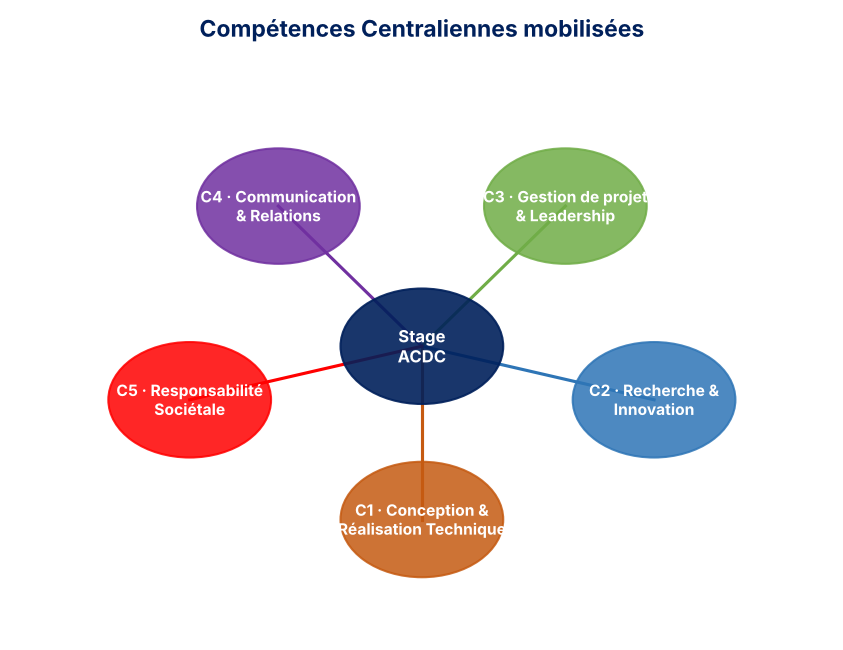
\includegraphics[width=0.6\textwidth]{competences_centraliennes}
  \caption{Les compétences centraliennes développées au cours du stage.}
  \label{fig:competences}
\end{figure}

\section{Diriger un programme : de la structuration à la réalisation autonome}

Dès les premiers jours du stage, j'ai dû définir un cadre méthodologique rigoureux pour garantir l'avance du projet. J'ai établi un diagramme de Gantt afin de jalonner les différentes phases~: recherche documentaire et prise en main des équipements, développement expérimental, puis optimisation, analyse et rédaction.

En parallèle, j'ai réalisé un reporting régulier auprès de mon tuteur, et présenté mes travaux devant l'ensemble des chercheurs lors des réunions bimensuelles de l'ACDC. Ces temps d'échange ont été essentiels pour recueillir des retours et ajuster certains choix méthodologiques.

\section{S'inscrire dans une vision stratégique collective}

Bien que mon projet ait été conduit en autonomie, j'ai été marqué par la vision stratégique portée par le Professeur Ziv Hameiri. L'ACDC Research Group cultive une culture de la cohésion où chacun s'inscrit dans une mission commune~: lutter contre le réchauffement climatique par le développement de l'énergie solaire.

\section{Créer de la valeur par l'innovation}

Le c\oe ur de mon stage a consisté à proposer une approche innovante pour une problématique expérimentale ouverte. Transposer une technique de mesure indoor vers un environnement outdoor a nécessité de sortir du cadre strict des protocoles établis et de faire preuve de créativité méthodologique.

\section{Maîtriser la complexité et agir en environnement incertain}

Travailler sur un sujet pluridisciplinaire mêlant physique des semi-conducteurs, optique, instrumentation et traitement du signal dans un environnement expérimental par nature variable m'a forcé à adopter une démarche rigoureuse et à quantifier les incertitudes.

\section{Manager de façon éthique et responsable}

Au-delà des aspects techniques, ce stage m'a permis de développer une conscience aiguë des enjeux environnementaux liés à la recherche en énergie solaire, renforçant ma conviction que l'ingénieur de demain doit être porteur d'une vision responsable.

Ce stage m'a permis de développer de manière concrète les compétences attendues d'un ingénieur centralien~: conduite de projet, autonomie, innovation, et capacité à évoluer dans des environnements complexes et interculturels.

% ── CONCLUSION GÉNÉRALE ────────────────────────────────────
\chapter*{Conclusion générale}
\addcontentsline{toc}{chapter}{Conclusion générale}

Ce stage de recherche de cinq mois, réalisé au sein de l'ACDC Research Group à l'UNSW, a constitué une expérience aussi exigeante qu'enrichissante. Il m'a permis d'explorer un domaine à la fois fondamental et expérimental à travers un projet conduit en autonomie dans un laboratoire de renommée internationale.

Les principaux résultats scientifiques sont~:
\begin{itemize}
  \item Optimisation numérique du filtre interférentiel ($\lambda_\text{CW} = 680$~nm, $\Delta\lambda = 30$~nm, $\sigma_{i\text{Voc}} = 1{,}8$~mV) par simulation Python sur 3\,136 combinaisons~;
  \item Calibration robuste par auto-étalonnage ($R^2 = 0{,}9994$, reproductibilité 1,1~mV sur la constante~$A$)~;
  \item Validation de la méthode OC$-$SC sur le terrain (UNSW Kensington, 4~juin~2025), avec une incertitude globale $\pm 2{,}1$~mV~;
  \item Détection d'une dégradation localisée sur la cellule n°2 (taux 1,6$\times$ supérieur aux autres), validant la sensibilité de la méthode pour le suivi de vieillissement.
\end{itemize}

Au-delà des compétences scientifiques et expérimentales consolidées, cette expérience m'a permis de développer une véritable posture d'ingénieur~: structurer un projet, faire des choix dans l'incertitude, communiquer ses résultats et s'inscrire dans une dynamique collective.

Le contexte international et l'ouverture du laboratoire sur les grands enjeux environnementaux m'ont permis de replacer mon travail dans un cadre plus large, porteur de sens. Ce stage constitue une étape importante dans mon parcours de formation.

% ── BIBLIOGRAPHIE ──────────────────────────────────────────
\printbibliography[heading=bibintoc,title={Bibliographie}]

% ── ANNEXES ────────────────────────────────────────────────
\appendix

\chapter{Protocole de mesure outdoor détaillé}

\begin{encadre}[title={Note}]
Cette annexe est à compléter avec les photos du dispositif expérimental et les détails du protocole de mesure.
\end{encadre}

\chapter{Scripts Python}

\section*{Simulation du choix des filtres}

\begin{verbatim}
import numpy as np
import matplotlib.pyplot as plt

# Paramètres de la grille
CW_range = np.arange(620, 905, 5)   # nm
BW_range = np.arange(5,  105, 5)    # nm
kT_q     = 25.7e-3                  # eV (25°C)

# Chargement spectres
# am15g = np.loadtxt('AM15G.csv', ...)
# qe_ingaas = np.loadtxt('QE_InGaAs.csv', ...)

# Calcul sigma_iVoc pour chaque (CW, BW)
sigma_map = np.zeros((len(BW_range), len(CW_range)))
for i, BW in enumerate(BW_range):
    for j, CW in enumerate(CW_range):
        # Filtre passe-bande (porte idéale)
        lam = np.linspace(CW-BW/2, CW+BW/2, 100)
        # S_PL = intégrale(Planck_generalise * QE)
        # S_sol = intégrale(AM15G * r * QE)
        # sigma_map[i,j] = kT_q * sqrt(S_sol) / S_PL * 1e3
        pass

plt.figure(figsize=(10, 6))
plt.pcolormesh(CW_range, BW_range, sigma_map,
               cmap='RdYlGn_r', vmin=0, vmax=10)
plt.colorbar(label=r'$\sigma_{iVoc}$ (mV)')
plt.xlabel('Longueur d\'onde centrale (nm)')
plt.ylabel('Bande passante (nm)')
plt.title(r'Erreur $\sigma_{iVoc}$ en fonction du filtre')
plt.tight_layout()
\end{verbatim}

\chapter{Données brutes des mesures PL outdoor}

\begin{encadre}[title={Note}]
Cette annexe est à compléter avec les spectres PL mesurés et les tableaux de valeurs d'$i$Voc extraites.
\end{encadre}

\end{document}
